
%\begin{figure}[t]
%\centering
%\includegraphics[scale=1,clip]{figure/n2n.eps}\vspace*{-3ex}
% \caption{Merging technique}\vspace*{-3.5ex}
% \label{fig:n2n}
%\end{figure}

\section{Discussion and Future Work}
\label{sec:discuss}

We next discuss issues in our approach and describe how we address
these issues in our future work.

\textbf{Testing API methods with no return values or random return values.} If an API method returns no values and throws no exceptions, TeMaAPI cannot generate any test cases for them to detect differences of their API mapping relations since it relies on comparing return values for detecting differences. We find that the FAQ of JUnit\footnote{\url{http://tinyurl.com/2ccsl5q}} also discusses a related issue. In this page, Dave Astels suggests to test side effects or to introduce mock objects for methods without return values. We plan to follow his advice in future work. In addition, we find that some API methods return random values, so we cannot conclude their mapped API methods have different behaviors even if corresponding JUnit test cases fail. To test such API methods, we plan to introduce other test oracles in future work. For example, we can generate many test cases and check whether mapped methods generate random values of the same ranges.

\textbf{Extracting invocation sequences from existing compatibility kit.} Although randomly generated invocation sequences reveal some different behaviors, these random invocation sequences may not reflect API usages in true practice. We notice that Java provides the Compatibility Kit (JCK)\footnote{\url{http://jck.dev.java.net}} to ensure the compatibility of Java provided by different vendors. Besides other requirements, JCK  defines many typical invocation sequences of API methods with their inputs and expected outputs. In future work, we plan to extract invocation sequences from such compatibility kit, and detect different behaviors based on extracted invocation sequences. 

\textbf{Testing code structures for migration tools.} We find that migration tools fail to translate some JUnit test cases since code structures are complicated. Developers of migration tools already notice some such code structures. For example, Java2CSharp lists some unsupported code structures in its website\footnote{\url{http://tinyurl.com/27z7qrj}}. It may be desirable if some approaches can detect these complicated code structures, so that migration tools can improve their translation capabilities. Daniel \emph{et al.}~\cite{daniel2007automated} propose an approach that tests refactory engines by comparing their refactored results given the same generated abstract syntax trees. The idea inspires our future work to testing code structures for migration tools by comparing the translation results given the same generated code snippets. 